\documentclass{article}
\usepackage{import}
\usepackage[backend = biber, style=authoryear, sorting=nyt]{biblatex}
\addbibresource{bibliography.bib}
\usepackage{mypreamble}

\title{Moses Illusion Experiment Report}
\author{Catarina Costa}
\date{June 29\textsuperscript{th}, 2024}

\begin{document}
\maketitle

\tableofcontents

\section{Moses Illusion}

\textit{How many animals of each kind did Moses take on the ark?} If you answered \enquote{two} to this question, you have fallen into the Moses illusion. According to \cite{ERICKSON1981540}, Moses Illusions or semantic illusions occur when readers fail to recognize the inconsistency in a text even if they were warned and know the correct word. In this case, you would have to be quick to realise that Noah took animals on the ark, not Moses.

\section{Experiment}
This experiment was conducted in the context of the class Digital Research Toolkit for Linguists, Summer Semester 2024, in order to gather data to then be analysed during class. In the experiment, the task was to:
\begin{itemize}
    \item Answer the questions in a questionnaire.
    \item Answer \enquote{don't know} if you didn't know the answer.
    \item Answer \enquote{can't answer} if a question seemed distorted or nonsensical.
\end{itemize}

An example question could be "Cairo is the capital of which African country?" and the corresponding answer is "Egypt". An example of an illusion question could be:

\Tree [.S This
[.VP [.V is ]
[.DP [.D a ]
\qroof{question:}.NP ] ] ]



\begin{exe}
\ex \begin{xlist}
\ex \gll How many fingers do fish have on their hind legs?\\
Quantos dedos têm os peixes nas suas pernas traseiras?\\
\end{xlist}
\end{exe}

To which the answer would be \enquote{can't answer}.

\subsection{Methods}
\subsubsection{Participants}
This experiment was shared with course participants, who then would have to recruit at least one more person to answer the experiment.
\subsubsection{Materials}
The experiment was prepared and organized by the teacher of this course, Anna Pryslopska. To take part in this study, it was necessary to have only a computer with a keyboard.

\subsubsection{Procedure}
The task\footnote{The actual procedure and experiment can be consulted \href{https://farm.pcibex.net/p/glQRwV/}{here}} in this experiment consisted of reading and answering questions, as explained in section \textbf{2. Experiment}. In figure \ref{fig:enter-label} we can see an example of how a question would appear to the user conducting the task.

\begin{figure}
    \centering
    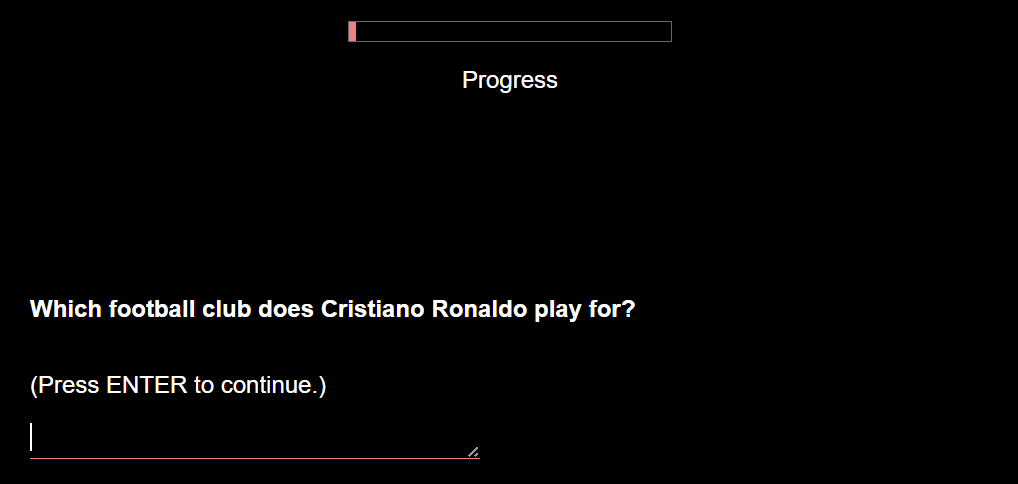
\includegraphics[width=1\linewidth]{mosesfigure.png}
    \caption{Overview of the experiment layout.}
    \label{fig:enter-label}
\end{figure}


\subsection{Predictions}
It could be expected that a lot of people would fall for the Moses Illusion, producing very interesting results.
In Table \ref{tab:my-label} are some of the results we saw:


\begin{table}
    \begin{tabular}{lcr}
         \textbf{Question} &\textbf{Finding} \\
         \hline
         Easiest Question &103 \\
         Hardest Question &17 \\
         Questions that fooled the most people &2 and 12 \\
         ID of best participant &880f21222ca0914d0b9f29de0e9cf92a \\
         ID of worst participant	&19c2d7b9ded0b515c030e3b36dd11909 \\
    \end{tabular}
    \caption{Questions and findings of the Moses Experiment.}\label{tab:my-label}
\end{table}

\subsection{Analysis and Results}
In class, using R and RStudio, we analysed the results of this experiment, as well as the reading time necessary for each participant.

\section{Discussion}

Why do people fall so easily into the Moses Illusions? This very interesting experiment already has a lot of research around it. For example, according to \parencite{doi:10.1080/09658211.2013.799701}, older adults fall for it more often. In this thesis\footcite{kups55556} and in \citetitle{speckmann2021moses}, Speckmann explores further motivations that might make the person more attentive and change their answers, continuing this work even in \citeyear{inbook}. \nocite{kahneman2011thinking}
\textcite{davis2016here} challenge theoretical explanations of the Moses illusion as resulting from purely shallow semantic processing and demonstrate the importance of visual information in processing proper names, even when presented in written form and \citeauthor{bottoms2010memory} explore the negative memorial consequences of the failures to detect these kind of contradictions with stored knowledge. \cite{raposo2013contribution} explores the Moses Illusion from a neuroscience perspective and \cite{izaute2004benzodiazepines} even digs into the effects that a specific kind of medication can have when conducting this experiment.
The fact remains, even in such a small group as a classroom, we could already prove how easily it is to fall for it.


\section{A Random Ending}

Here is a semantic formula, because why not:
\[
\models (P \land Q) \rightarrow R
\]

\printbibliography

\end{document}
